\documentclass[12pt]{article}

\input quiz-setup
\newcommand{\version}{} 
\newcommand{\xzero}{}
\newcommand{\xone}{}
\newcommand{\xtwo}{}
\newcommand{\xthree}{}
\newcommand{\xfour}{}
\newcommand{\xfive}{}

\newcommand{\ExamName}{Quiz \#3\version}
% \newcommand{\CourseName}{Math 34A}
% \renewcommand{\Quarter}{Spring 2017}





\begin{document}
%%
%% Version A:
\renewcommand{\version}{}
\renewcommand{\xzero}{0.0}
\renewcommand{\xone}{1.3}
\renewcommand{\xtwo}{2.9}
\renewcommand{\xthree}{4.1}
\renewcommand{\xfour}{5.3}
\renewcommand{\xfive}{6.5}
% 
\begin{minipage}{0.25\linewidth}
  \CourseName\ \Quarter \\
  \ExamName \\[1em]
  \textbf{No calculators}\\[2em]
\end{minipage}
\hfill
\begin{minipage}[t]{0.4\linewidth}
  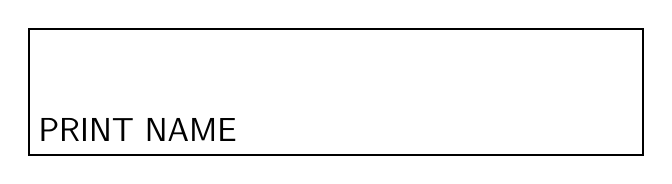
\begin{tikzpicture}[x=26mm,y=16mm]
    \draw[thick,black] (0,0) rectangle (3,1);
    \node[\faintcolor,right] at (0,0.2) {\large\textsf{PRINT NAME}};
  \end{tikzpicture}
\end{minipage}
\hfill
\begin{minipage}{0.25\linewidth}
  \vspace*{-3.25em}
  \ \hfill
  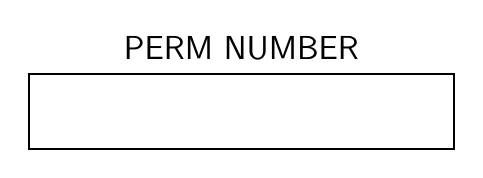
\begin{tikzpicture}[x=36mm,y=16mm]
    \node[\faintcolor] at (0.75,0.8) {\large\textsf{PERM NUMBER}};
    \draw[thick,black] (0,0) rectangle (1.5,0.6);
  \end{tikzpicture}
\end{minipage}
% \medskip
\vspace*{-0.25in}

Put your answer in the 
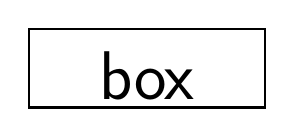
\begin{tikzpicture}[x=10mm,y=10mm,baseline=3mm] 
  \draw[thick,black] (0,0) rectangle (3,1);
  \node[\faintcolor] at (1.5,0.4) {\Huge\textsf{box}};
\end{tikzpicture}
provided.
\hfill
\begin{minipage}{0.5\linewidth}
\begin{center}

  \textbf{TA:}\ 
  \parbox[t]{0.7in}{%
    \checkbox\ \TAOne \\
    \checkbox\ \TATwo 
  }
  %\parbox[t]{0.7in}{%
  %  \checkbox\ \TAThree\\
  %  \ \ \ 
  %}
  % \ 
  % \parbox[t]{4in}{%
  % \textbf{Section Time:}
  \hfill%\hspace*{0.25in}
  % \ 
  % \parbox[t]{4in}{%
  % \textbf{Section Time:}
  \textbf{Time:}
  \parbox[t]{0.55in}{%
    \checkbox\ 4:30 \\
    \checkbox\ 5:30
  }
  \quad
  \parbox[t]{0.55in}{%
    \checkbox\ 6:30 \\
    \checkbox\ 7:30 
  }
  % }
%  \textbf{TA:}\ 
%  \parbox[t]{0.95in}{%
%    \checkbox\ \TAOne
%  }
%  \parbox[t]{0.95in}{%
%    \checkbox\ \TATwo\\
%  }
%%  \parbox[t]{0.95in}{%
%%    \checkbox\ \TAThree
%%  }
%  \hspace*{0.5in} 
%  \parbox[t]{3in}{%
%    \textbf{Section Time:}
%    \parbox[t]{0.75in}{%
%      \checkbox\ 4:30 \\
%      \checkbox\ 5:30
%    }
%    \parbox[t]{0.75in}{%
%      \checkbox\ 6:30 \\
%      \checkbox\ 7:30
%    }
%  }
\end{center}

\end{minipage}
\noindent\hspace*{-2em}\rule{\textwidth+4em}{1pt}%

\begin{enumerate}
  \setcounter{problemnumber}{0}
  
	\Problem What is the keyword? \answerbox{6}

	\bigskip
  
  \Problem 
 Consider the following homogeneous second-order differential equation with constant coefficients: \[4y''+by'+y = 0\] Consider $b$ to be a constant whose value we will decide later. 
 
 \begin{enumerate}
 \item Solve the characteristic equation in terms of b. 

		\begin{flushright}
		$r=$ 
		\begin{tikzpicture}[x=10mm,y=10mm,baseline=11mm] 
	  \draw[thick,black] (0,0) rectangle (6,2.5);
	  \node[\faintcolor] at (1.5,0.4) {};
		\end{tikzpicture}
		\end{flushright}
 
 		\vfill
 
 \item Choose three different values of $b$ such that the fundamental solution sets are distinct. [Hint: Choosing $b$ so that the discriminant is a whole number gives you 3 very nice values.]
 
 	 	\begin{itemize}
 	 		\item[] $b=$ \answerbox{2} \quad $y_1=$ \answerbox{3} \quad $y_2=$ \answerbox{3}
			\bigskip
			
			\item[] $b=$ \answerbox{2} \quad $y_1=$ \answerbox{3} \quad $y_2=$ \answerbox{3}
			\bigskip
			
			\item[] $b=$ \answerbox{2} \quad $y_1=$ \answerbox{3} \quad $y_2=$ \answerbox{3}
			\bigskip
 	 	\end{itemize}
 
 \end{enumerate}
  
  \vfill
  
  \newpage
  
  \Problem   
  This will introduce you to the idea behind a topic in the upcoming week(s). For each of the following functions, find 
  \[3y''+y'-2y.\] 
  
		\begin{enumerate}
		\item $y(t)=3e^t$
			\begin{flushright} $3y''+y'-2y=$ \answerbox{3} \end{flushright}
		\vfill			
		
		\item $y(t)=3t^2+5t-2$
			\begin{flushright} $3y''+y'-2y=$ \answerbox{3} \end{flushright}
		\vfill
		
		\item $y(t)=4\sin(t)$
			\begin{flushright} $3y''+y'-2y=$ \answerbox{3} \end{flushright}
		\vfill
		
		\item $y(t)=7\cos(t)$		
			\begin{flushright} $3y''+y'-2y=$ \answerbox{3} \end{flushright}
		\vfill
		
		\end{enumerate}	
		
	\pagebreak	
	\Problem Notice how in the previous problem, the functions remained the same type: exponentials, polynomials, trig functions, etc. Let's use this observation to find a particular solution to the \textbf{non}homogeneous equation
	$$y''-3y'-4y=3e^{2t}.$$
		\begin{enumerate}
		\item Let $y(t)=Ae^{2t}$, and consider $A$ to be a constant whose value we will decide later. Plug $y$ into the differential equation. 
			\vspace*{-12pt}
			\begin{flushright} $y''-3y'-4y=$ \answerbox{3} \end{flushright}
		\vfill
		
		\item Find the value of $A$ so that your answer to (a) is equal to $3e^{2t}$. 
			\begin{flushright} $A=$ \answerbox{2} \end{flushright}
		\vfill
		
		\item Check that $Ae^{2t}$ (with your value from part (b) plugged in) is a solution to $y''-3y'-4y=3e^{2t}.$
		\vfill
		\end{enumerate}
	\vfill
	
  

\end{enumerate}

\end{document}
